\documentclass[]{article}
\usepackage{lmodern}
\usepackage{amssymb,amsmath}
\usepackage{ifxetex,ifluatex}
\usepackage{fixltx2e} % provides \textsubscript
\ifnum 0\ifxetex 1\fi\ifluatex 1\fi=0 % if pdftex
  \usepackage[T1]{fontenc}
  \usepackage[utf8]{inputenc}
\else % if luatex or xelatex
  \ifxetex
    \usepackage{mathspec}
  \else
    \usepackage{fontspec}
  \fi
  \defaultfontfeatures{Ligatures=TeX,Scale=MatchLowercase}
\fi
% use upquote if available, for straight quotes in verbatim environments
\IfFileExists{upquote.sty}{\usepackage{upquote}}{}
% use microtype if available
\IfFileExists{microtype.sty}{%
\usepackage{microtype}
\UseMicrotypeSet[protrusion]{basicmath} % disable protrusion for tt fonts
}{}
\usepackage{hyperref}
\hypersetup{unicode=true,
            pdfborder={0 0 0},
            breaklinks=true}
\urlstyle{same}  % don't use monospace font for urls
\usepackage{longtable,booktabs}
\usepackage{graphicx,grffile}
\makeatletter
\def\maxwidth{\ifdim\Gin@nat@width>\linewidth\linewidth\else\Gin@nat@width\fi}
\def\maxheight{\ifdim\Gin@nat@height>\textheight\textheight\else\Gin@nat@height\fi}
\makeatother
% Scale images if necessary, so that they will not overflow the page
% margins by default, and it is still possible to overwrite the defaults
% using explicit options in \includegraphics[width, height, ...]{}
\setkeys{Gin}{width=\maxwidth,height=\maxheight,keepaspectratio}
\IfFileExists{parskip.sty}{%
\usepackage{parskip}
}{% else
\setlength{\parindent}{0pt}
\setlength{\parskip}{6pt plus 2pt minus 1pt}
}
\setlength{\emergencystretch}{3em}  % prevent overfull lines
\providecommand{\tightlist}{%
  \setlength{\itemsep}{0pt}\setlength{\parskip}{0pt}}
\setcounter{secnumdepth}{0}
% Redefines (sub)paragraphs to behave more like sections
\ifx\paragraph\undefined\else
\let\oldparagraph\paragraph
\renewcommand{\paragraph}[1]{\oldparagraph{#1}\mbox{}}
\fi
\ifx\subparagraph\undefined\else
\let\oldsubparagraph\subparagraph
\renewcommand{\subparagraph}[1]{\oldsubparagraph{#1}\mbox{}}
\fi

\date{}

\begin{document}

\section{PERSONAL INFORMATION}\label{personal-information}

\emph{Name} Jose Nuno de Pinho Cardoso\\
Date of Birth 27-05-1988\\
Place of Birth Porto\textbackslash{}Portugal\\
Nationality \textbf{Portuguese}\\
Citizen Card ID 13216754

\begin{center}\rule{0.5\linewidth}{\linethickness}\end{center}

\section{EDUCATIONZ}\label{educationz}

\subsubsection{Escola superior do MIEIC}\label{escola-superior-do-mieic}

\begin{longtable}[c]{@{}lll@{}}
\toprule
Disciplina & Professor & Score\tabularnewline
\midrule
\endhead
ASSO & LFR & a\tabularnewline
COMP & Luis RUi & 17\tabularnewline
\bottomrule
\end{longtable}

\subsection{Universidade}\label{universidade}

\begin{longtable}[c]{@{}rll@{}}
\toprule
\begin{minipage}[b]{0.06\columnwidth}\raggedleft\strut
Disciplina
\strut\end{minipage} &
\begin{minipage}[b]{0.05\columnwidth}\raggedright\strut
Professor
\strut\end{minipage} &
\begin{minipage}[b]{0.06\columnwidth}\raggedright\strut
Stars
\strut\end{minipage}\tabularnewline
\midrule
\endhead
\begin{minipage}[t]{0.06\columnwidth}\raggedleft\strut
LGP
\strut\end{minipage} &
\begin{minipage}[t]{0.05\columnwidth}\raggedright\strut
~~~~~
\strut\end{minipage} &
\begin{minipage}[t]{0.06\columnwidth}\raggedright\strut

\includegraphics{file:/C:/Users/david/OneDrive/Documentos/FEUP/3Ano/COMP/MCV/build/classes/filled.png}
\includegraphics{file:/C:/Users/david/OneDrive/Documentos/FEUP/3Ano/COMP/MCV/build/classes/filled.png}
\includegraphics{file:/C:/Users/david/OneDrive/Documentos/FEUP/3Ano/COMP/MCV/build/classes/filled.png}
\includegraphics{file:/C:/Users/david/OneDrive/Documentos/FEUP/3Ano/COMP/MCV/build/classes/filled.png}
\includegraphics{file:/C:/Users/david/OneDrive/Documentos/FEUP/3Ano/COMP/MCV/build/classes/filled.png}
\includegraphics{file:/C:/Users/david/OneDrive/Documentos/FEUP/3Ano/COMP/MCV/build/classes/half-star.png}
\includegraphics{file:/C:/Users/david/OneDrive/Documentos/FEUP/3Ano/COMP/MCV/build/classes/empty.png}
\includegraphics{file:/C:/Users/david/OneDrive/Documentos/FEUP/3Ano/COMP/MCV/build/classes/empty.png}
\includegraphics{file:/C:/Users/david/OneDrive/Documentos/FEUP/3Ano/COMP/MCV/build/classes/empty.png}
\includegraphics{file:/C:/Users/david/OneDrive/Documentos/FEUP/3Ano/COMP/MCV/build/classes/empty.png}
\includegraphics{file:/C:/Users/david/OneDrive/Documentos/FEUP/3Ano/COMP/MCV/build/classes/empty.png}
\includegraphics{file:/C:/Users/david/OneDrive/Documentos/FEUP/3Ano/COMP/MCV/build/classes/empty.png}
\strut\end{minipage}\tabularnewline
\bottomrule
\end{longtable}

\section{Lista De linguagens}\label{lista-de-linguagens}

\begin{enumerate}
\tightlist
\item
  Java
\item
  C
\item
  Jade
\end{enumerate}

\section{Lista de Gostos}\label{lista-de-gostos}

\begin{itemize}
\tightlist
\item
  Web
\item
  SQL
\end{itemize}

\section{QUOTES}\label{quotes}

\begin{quote}
Melhor empregado que ja tive\\
Sinceramente fantastico\\
Excelente Aluno
\end{quote}

\section{LINKS E IMAGENS}\label{links-e-imagens}

{[}www.google.com{]}\\
\includegraphics{/C.NOmeuDisco.png}

\section{WORDCLOUD}\label{wordcloud}

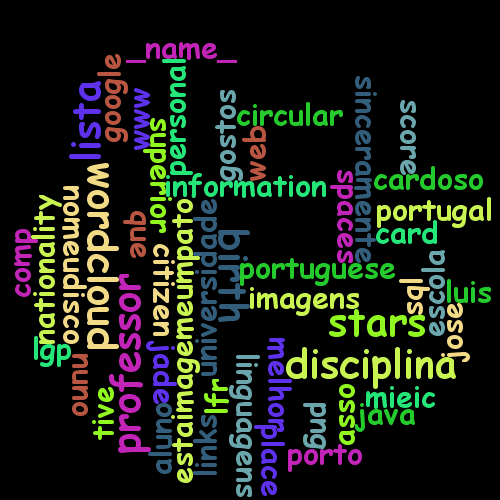
\includegraphics{C:/Users/david/OneDrive/Documentos/FEUP/3Ano/COMP/MCV/Output/customwordcloud.png?raw=true}

\end{document}
